\documentclass[tikz,border=3pt]{standalone}
\usepackage{fontspec}
\usepackage{amsmath}
\usepackage{xcolor}
\usepackage{tikz}
\usepackage{pgfplots}
\pgfplotsset{compat=1.18}
\usetikzlibrary{arrows.meta,calc,fit,positioning,shapes.geometric,shapes.misc,patterns,plotmarks}
\IfFontExistsTF{Arial}{\setsansfont{Arial}}{\setsansfont{TeX Gyre Heros}}
\renewcommand{\familydefault}{\sfdefault}
\tikzset{
  >={Stealth[length=2.2mm,width=1.5mm]},
  exact title/.style={font=\bfseries\fontsize{10.5}{12}\selectfont,align=center},
  exact subtitle/.style={font=\fontsize{6.3}{7.2}\selectfont,align=center},
  exact label/.style={font=\fontsize{6.4}{7.5}\selectfont,align=center},
  exact tiny/.style={font=\fontsize{5.3}{6.3}\selectfont,align=center},
  panel/.style={draw=black!14,rounded corners=1.2mm,fill=white,line width=.45pt},
  neutral/.style={draw=black!30,fill=black!3,rounded corners=1mm,line width=.45pt},
  arrow/.style={-Stealth,line width=.7pt},
  softarrow/.style={-Stealth,line width=.55pt,draw=black!45},
  dashedarrow/.style={-Stealth,dashed,line width=.55pt,draw=black!55},
  metric/.style={font=\fontsize{5.3}{6.3}\selectfont,fill=white,inner sep=1pt},
}
\newcommand{\pill}[4]{\node[draw=#2!70,fill=#2!10,rounded corners=1.5mm,inner xsep=3pt,inner ysep=2pt,exact label,text=#2] (#1) at #3 {#4};}
\newcommand{\frameboxx}[4]{\draw[draw=#2!65,fill=#2!8,rounded corners=.6mm,line width=.5pt] (#1.south west) rectangle (#1.north east);\node[exact tiny,text=#2] at #3 {#4};}
\newcommand{\axislabel}[3]{\node[exact tiny,text=black!60] at (#1) {#2};\node[exact tiny,text=black!60,rotate=90] at (#3) {#2};}

\definecolor{exblue}{HTML}{3568A8}\definecolor{exorange}{HTML}{E98B4A}\definecolor{exgray}{HTML}{9AA3AF}\definecolor{exgreen}{HTML}{4C956C}\definecolor{exink}{HTML}{263238}
\begin{document}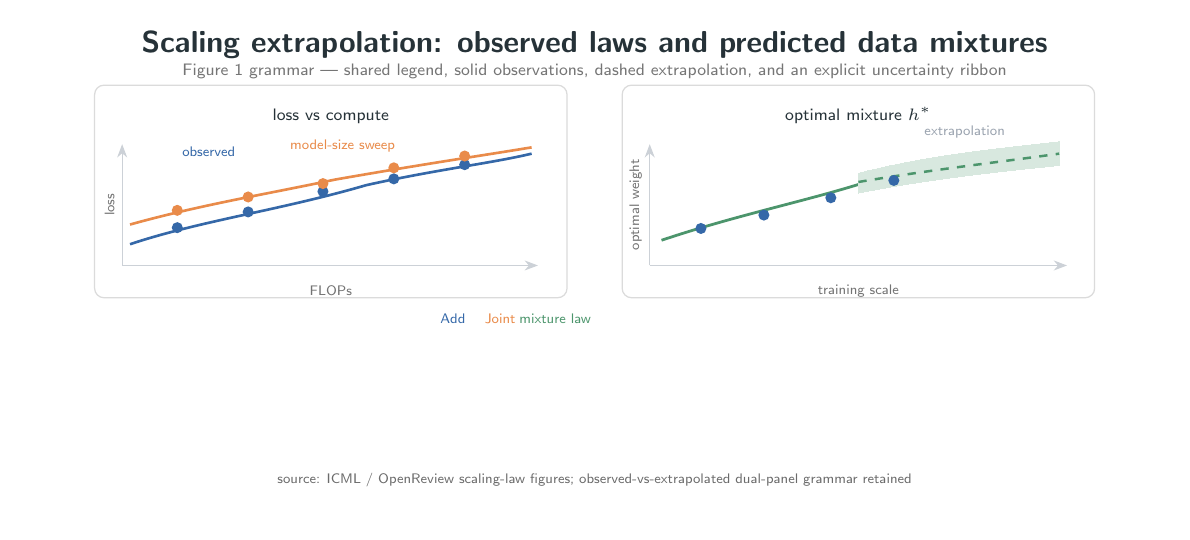
\begin{tikzpicture}[x=1cm,y=1cm]
\path[use as bounding box] (-.2,-3.95) rectangle (14.2,2.2);
\node[exact title,text=exink] at (7,1.98) {Scaling extrapolation: observed laws and predicted data mixtures};
\node[exact subtitle,text=black!54] at (7,1.64) {Figure 1 grammar — shared legend, solid observations, dashed extrapolation, and an explicit uncertainty ribbon};
\node[panel,minimum width=6.0cm,minimum height=2.7cm] at (3.65,.12) {};
\node[panel,minimum width=6.0cm,minimum height=2.7cm] at (10.35,.12) {};
\node[exact label,text=exink] at (3.65,1.08) {loss vs compute};\node[exact label,text=exink] at (10.35,1.08) {optimal mixture \(h^*\)};
\draw[exgray!50,-Stealth] (1.0,-.82) -- (6.28,-.82);\draw[exgray!50,-Stealth] (1.0,-.82) -- (1.0,.72);\draw[exblue,line width=.95pt] (1.1,-.55) .. controls (2.0,-.25) and (3.0,-.12) .. (4.1,.2) .. controls (5.0,.4) and (5.7,.48) .. (6.2,.6);\draw[exorange,line width=.95pt] (1.1,-.3) .. controls (2.0,-.05) and (2.8,.08) .. (3.7,.27) .. controls (4.9,.48) and (5.6,.58) .. (6.2,.68);\foreach \x/\y in {1.7/-.34,2.6/-.14,3.55/.12,4.45/.28,5.35/.46}{\fill[exblue] (\x,\y) circle (2pt);}\foreach \x/\y in {1.7/-.12,2.6/.05,3.55/.22,4.45/.42,5.35/.57}{\fill[exorange] (\x,\y) circle (2pt);}\node[exact tiny,text=exblue] at (2.1,.62) {observed};\node[exact tiny,text=exorange] at (3.8,.7) {model-size sweep};\node[exact tiny,text=black!55] at (3.65,-1.14) {FLOPs};\node[exact tiny,text=black!55,rotate=90] at (.84,-.05) {loss};
\draw[exgray!50,-Stealth] (7.7,-.82) -- (13.0,-.82);\draw[exgray!50,-Stealth] (7.7,-.82) -- (7.7,.72);\draw[exgreen,line width=1pt] (7.85,-.5) .. controls (8.8,-.18) and (9.7,.0) .. (10.45,.24) .. controls (11.3,.38) and (12.2,.5) .. (12.9,.6);\draw[exgreen!22,line width=0pt,fill=exgreen!22] (10.35,.1) .. controls (11.2,.27) and (12.1,.37) .. (12.9,.45) -- (12.9,.75) .. controls (12.0,.65) and (11.2,.57) .. (10.35,.35) -- cycle;\draw[exgreen,dashed,line width=.9pt] (10.35,.24) .. controls (11.3,.4) and (12.2,.5) .. (12.9,.6);\foreach \x/\y in {8.35/-.35,9.15/-.18,10.0/.04,10.8/.26}{\fill[exblue] (\x,\y) circle (2pt);}\node[exact tiny,text=exgray] at (11.7,.88) {extrapolation};\node[exact tiny,text=black!55] at (10.35,-1.14) {training scale};\node[exact tiny,text=black!55,rotate=90] at (7.52,-.05) {optimal weight};
\node[exact tiny,text=exblue] at (5.2,-1.5) {Add};\node[exact tiny,text=exorange] at (5.8,-1.5) {Joint};\node[exact tiny,text=exgreen] at (6.5,-1.5) {mixture law};
\node[exact tiny,text=black!58] at (7,-3.55) {source: ICML / OpenReview scaling-law figures; observed-vs-extrapolated dual-panel grammar retained};
\end{tikzpicture}\end{document}
